%!TEX root = main.tex

\section{Introduction}
\label{sec:intro}

\begin{figure}[ht]
	\centering
	%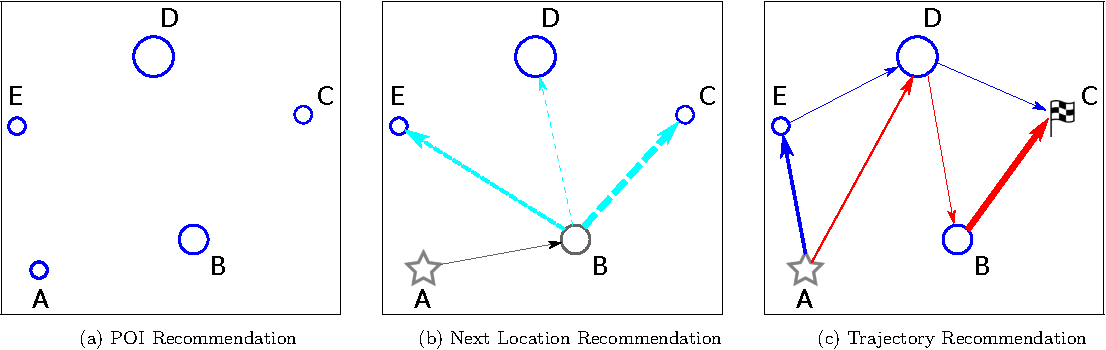
\includegraphics[width=0.7\textwidth]{fig/fig1-flavours.pdf}
	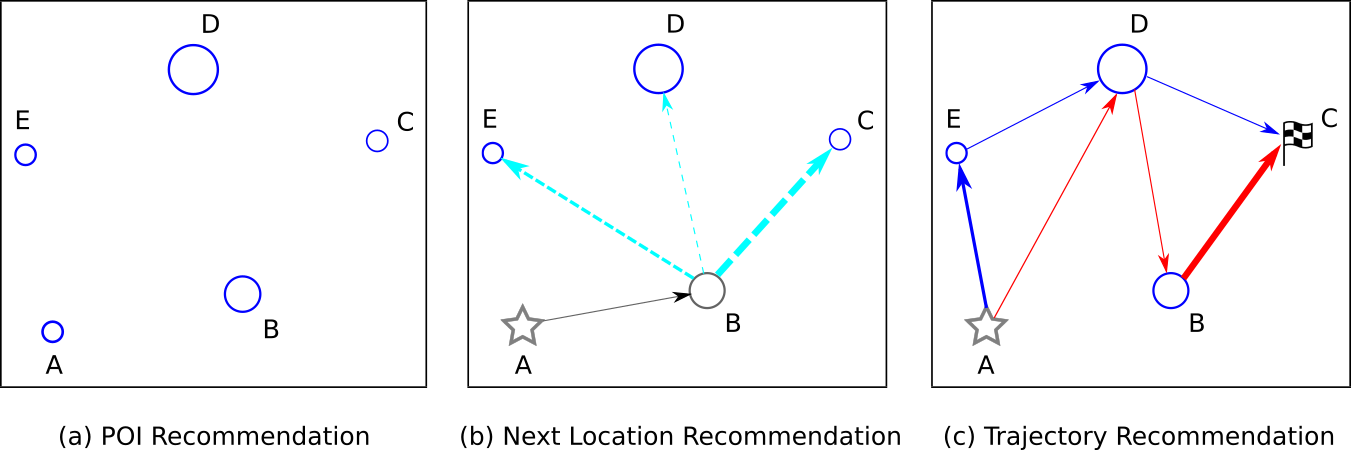
\includegraphics[width=\columnwidth]{fig/fig1-flavours.png}
	\caption{Three settings of trajectory recommendation problems. 
Node size: POI score; edge width: transition score between pairs of POIs; 
%grey: input query; 
grey: observed;
star: starting location; flag: ending location. See Section~\ref{sec:intro} for details.
}
	\label{fig:threesettings}
\end{figure}



This paper proposes a novel solution to recommend travel routes in cities.
A large amount of location traces are becoming available from ubiquitous location tracking devices.
For example, FourSquare
%, the local search and discovery service, 
has 50 million monthly users who have made 8 billion check-ins~\cite{4sq},
and Flickr
%, the online photo-sharing site, 
hosts over 2 billion geo-tagged public photos~\cite{flickr}. 
Such large amounts of travel data provide new opportunities for better
travel planning traditionally done with written travel guides.
%for example, choosing and ranking locations for a variety of activities from dining to recreation,
%and potential new solutions to orienteering and routing problems.
Good solutions to these problems will in turn lead to better urban experiences for residents and visitors alike, and foster sharing of even more location-based behavioural data.
